%%%%
% -- Schedule and Budget breakdown and funding path
% --     FOBOS Keck White Paper 2019
%%%%

\section{Schedule, Budget, and Funding Path}
\label{sec:budget}

\subsection{Funding Path}

Early funding for FOBOS has been obtained through a number of sources.
First, conceptual development of Fiber-WFOS for TMT has provided the
backbone for the current FOBOS design. Second, a number of smaller
grants were used to develop and assess specific aspects of FOBOS.
Namely, a 2016 UCO mini-grant (\$10k) to KG Lee was used for initial
collaboration development; a 2017 UCO mini-grant (\$25k) to KG Lee was
used for conceptual development of the microlens fore-optics; a 2017 UCO
mini-grant (\$55k) to K. Bundy allowed for a study of sky-subtraction
fidelity in existing fiber systems; WMKO white-paper funds (\$40k)
provided to K. Bundy in 2018 are still being used to develop science
cases, build invested science teams, and perform focal-plane and
spectrograph design studies; and a 2018 UCO mini-grant (\$120k) to K.
Bundy was provided for design and fabrication of a microlens-coupled
fiber system primarily to demonstrate its throughput at Keck compared to
lab measurements and to simultaneous observations with DEIMOS. The
latter builds on UCO's ongoing investment in a fiber-testing facility
needed for a number of internal projects has helped to further the FOBOS
design. This Phase A funding request is designed to bring the project to
a stage of readiness needed to submit proposals to the NSF MSIP (2020)
and MsRI-2 (2023) programs.

We intend to propose for FOBOS design funds via an MSIP solicitation
expected in early 2020; if successful, this will fund the full
instrument-design phase. The construction funding would then come
from a MsRI-2 proposal in 2023. We have requested ``Phase A'' funding
from late 2019 to mid 2021 to allow for continued development between
submitting our MSIP proposal and when the funding is made available.
In the event that we are unsuccessful in the MSIP proposal, our
requested ``Phase A'' funding in the last half of this proposal would
be used for preparation towards a MsRI-1 proposal in 2021. The
included schedule shows our NSF funding plan as funding windows at
the top of the Gantt chart.

We intend to apply for other smaller funding opportunities as they
become available, including the UCO mini-grant and NSF ATI grants.
Both of these would be targeted at relatively self-contained design
components of FOBOS's overall system. Other government funding and
private funding is also being pursued as opportunities become
available.

\begin{table}[h!]
\centering
\footnotesize
\caption{FOBOS Development Milestones}
\label{tab:milestones}
\vspace*{-10pt}
\begin{tabular}{l r r}
Milestone                     & Funding Level & Dates \\
\hline
\hline
CoD Mini Grant I              &  \$10k & FY2016 \\
CoD Mini Grant II             &  \$25k & FY2017 \\
CoD Mini Grant III            &  \$55k & FY2017 \\
LBNL workshop                 &        & 18 Jan 2018 \\
UCLA workshop                 &        & 4 May 2018 \\
WMKO Design                   &  \$40k & 8 Jun 2018 \\
WMKO Design Funding Window    &        & 1 Dec 2018 -- 30 Nov 2019 \\
CoD Mini Grant IV (FIDDLES)   & \$120k & FY2019 \\
FIDDLES Funding Window        &        & 10 Jan 2019 -- 11 Dec 2019 \\
\hline
MSRI-1 Proposal               &        & 19 Feb 2019 \\
WMKO Phase A                  & \$376k & 8 Jun 2019 \\
WMKO Phase A Funding Window   &        & 23 Sep 2019 -- 23 Jul 2021 \\
\hline
MSIP 2020 LOI, Pre-Proposal   &        & 1 Sep -- 18 Nov 2019 \\
MSIP 2020 Full Proposal       &   \$5M & 17 Apr 2020 \\
MSIP Funding Window           &        & 2 Apr 2021 -- 5 Dec 2024 \\
\hline
MSRI-2 LOI, Pre-Proposal      &        & 16 Feb -- 13 Mar 2023 \\
MSRI-2 Full Proposal          & $>$\$20M & 4 Aug 2023 \\
MSRI-2 Funding window         &        & 1 Aug 2024 -- 31 Sep 2028 \\
\hline
\end{tabular}
\end{table}

\newpage

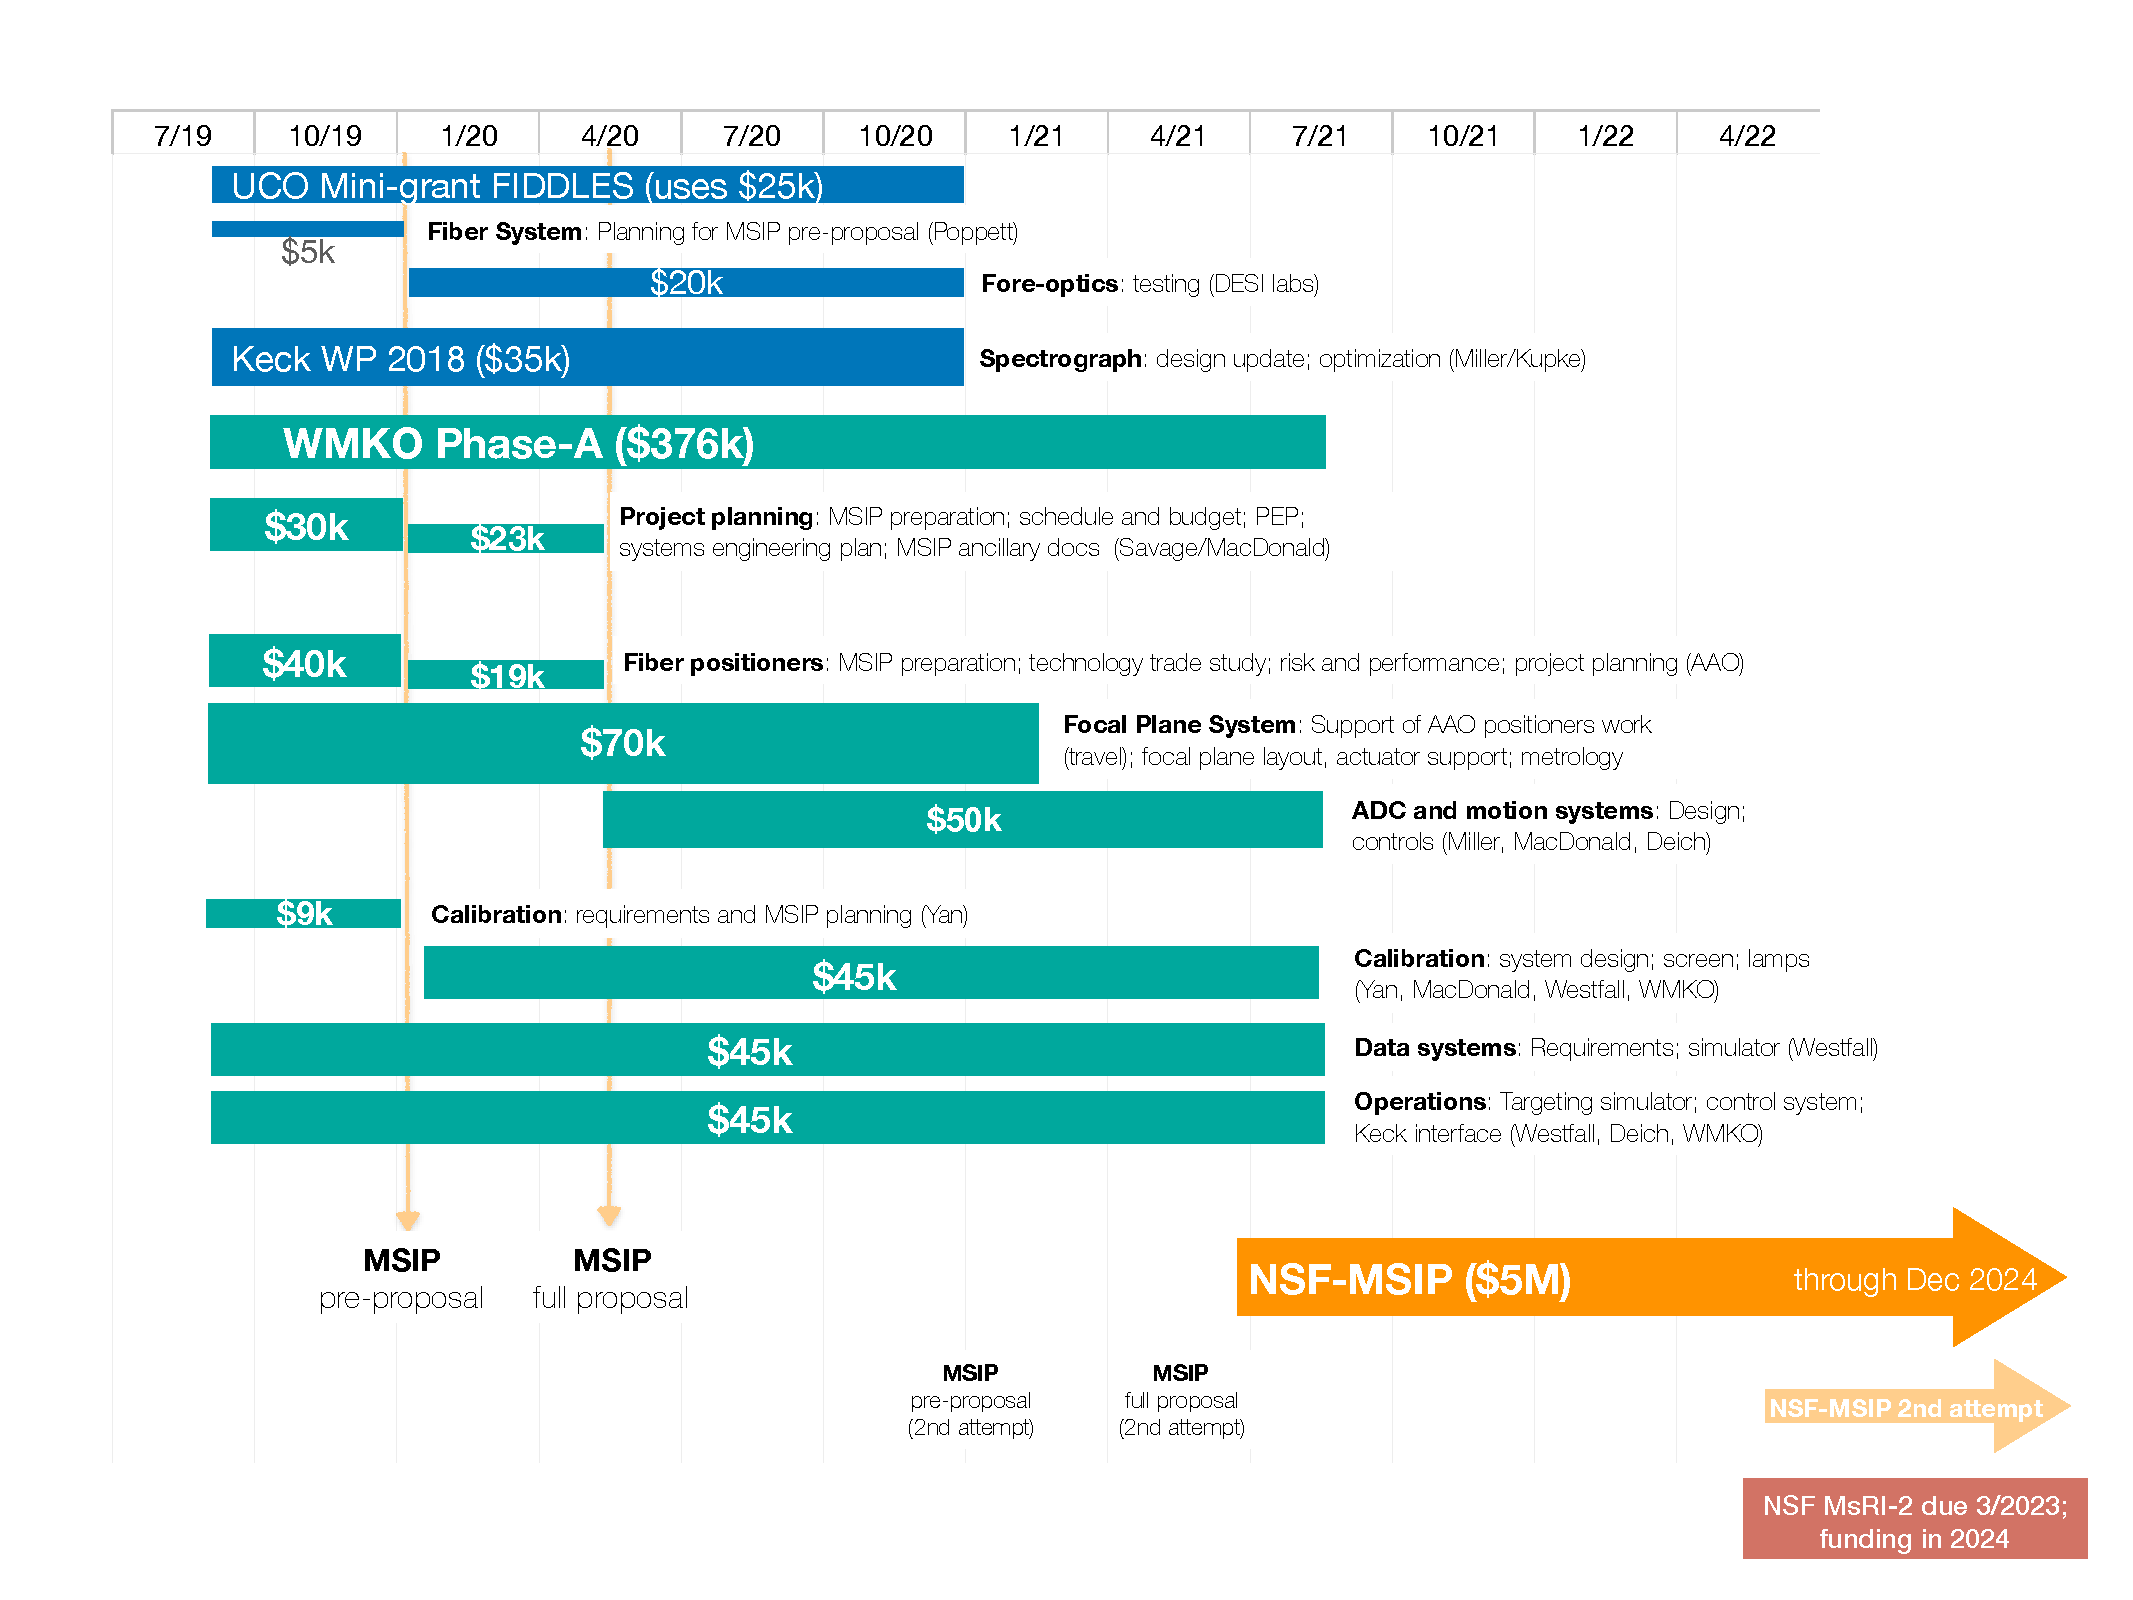
\includepdf[landscape=true]{figs/budget_schedule_schematic_v2.pdf}





